
\chapter{The Large Hadron Collider and the ATLAS Detector}
\label{ch:LHCDetector}

This chapter details the experimental details of the collider complex at the LHC and specifically the ATLAS detector used to produce, collect, and measure various particle properties.  The subsystems of the ATLAS detector are described in detail.
\section{The Large Hadron Collider}
\label{Section:LHC}
The LHC is the world's largest and most energetic particle accelerator.  As a hadron collider the LHC collides particles made up of quarks, typically proton-proton collisions.  Protons, as opposed to electrons/positrons at a previous collider such as LEP, have much higher mass and have a significantly smaller amount of energy loss during acceleration due to synchrotron radiation (which scales as $\frac{1}{m^4}$).  Due to this the LHC is able to reach a much higher center of mass energy using the same circular ring used by LEP.  
This higher energy comes at a cost though.  Due to hadrons being made up of constituent partons (quarks and gluons) not all of which interact in any given collision the particles that dont take place in the hard interaction are left over and create a 'messier' environment in the detectors.  Whereas in lepton colliders all of the energy that goes into the collision is present in the final state particles coming from the interaction point.  The implication of this is that hadron colliders cannot known the momentum along the beam axis and only know the momentum in the transverse plane due to conservation of momentum.

\begin{figure}[h!]
	\centering
	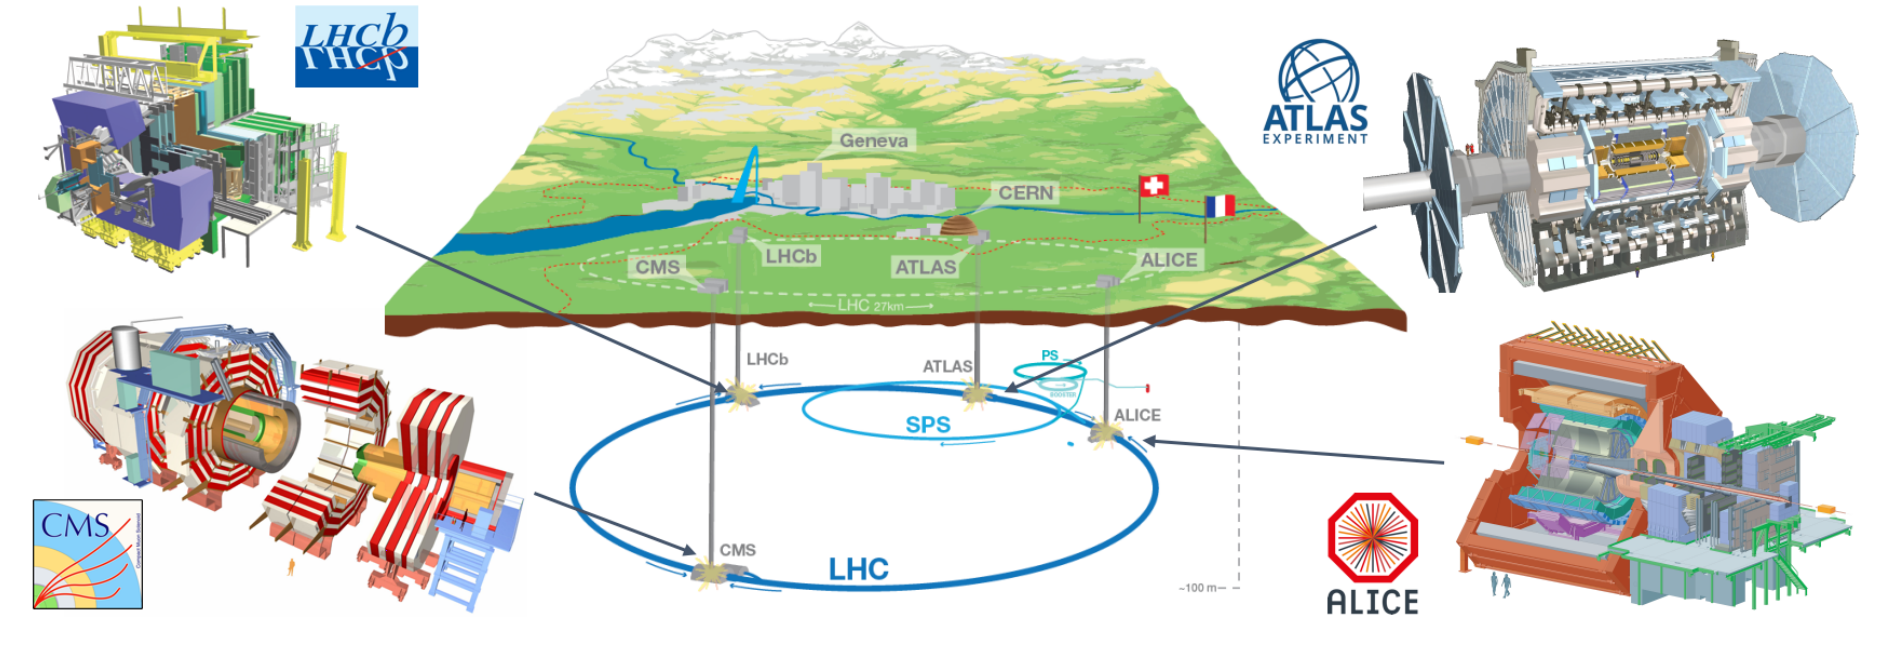
\includegraphics[width=\columnwidth]{../ThesisImages/LHCImages/LHCDetecPlacement.png}
	\caption[Map of LHC and the various detector experiments: ATLAS, CMS, LHCb, and ALICE located under the Franco-Swiss border near Geneva]{Map of LHC and the various detector experiments: ATLAS, CMS, LHCb, and ALICE  located under the Franco-Swiss border near Geneva\cite{ATLASCoords}}
	\label{fig:LHCDetPlace}
\end{figure}

The LHC is housed in a 27 km ring running beneath the Franco-Swiss border near Geneva, Switzerland and accelerates beams of protons (ions) to a center of mass energy of 13 TeV (5 TeV) using two counterpropagating circular beams around the ring.  The particles are then collided at one of the four primary interaction points, each of which house a dedicated detector as shown in Figure \ref{fig:LHCDetPlace}. 

In addition to the LHC beam line the accelerator uses a series of smaller accelerators to increase the energy of the particles before being introduced into the LHC.  This accelerator complex is detailed in Figure \ref{fig:AcceleratorMap}.  The start of the accelerator chain, and source of LHC protons, is the Linear Accelerator 2 (LINAC 2, purple) where hydrogen gas is placed inside of an electric field which separates the protons and electrons.  The remaining protons are passed through radiofrequency (RF) cavities and accelerated to 50 MeV using electric fields which oscillate at a frequency specific to the distance between any two RF cavities.
\begin{figure}[h!]
	\centering
	\includegraphics[width=\columnwidth]{../ThesisImages/LHCImages/AcceleratorComplex.png}
	\caption[Schematic of the CERN accelerator complex.]{Schematic of the CERN accelerator complex.\cite{LHCAccComplex}
	}
	\label{fig:AcceleratorMap}
\end{figure}

After leaving LINAC 2 the protons are injected into the Proton Synchrotron Booster (BOOSTER, light purple) and accelerated to 1.4 GeV before being passed to the Proton Synchrotron (PS, magenta) in two batches with a separation of 1.2 seconds.  The PS accelerates the protons to 25 GeV to be injected into the Super Proton Synchrotron (SPS, blue) in a series of four batches seperated by 3.6 seconds and are accelerated to 450 GeV.  The SPS is the second largest accelerator in the complex.  After being reaching the 450 GeV of the SPS the particles are split and injected into the LHC in opposing directions where they are further accelerated to a collision energy of 6.5 TeV per beam leading to a center of mass energy of 13 TeV for the LHC during Run-2.

The first proton-proton collisions were produced in the LHC in 2008 at the injection energy of the SPS, $\sqrt{s} =900$ GeV.  During testing a faulty electrical connection caused a magnet quench, a sudden loss of superconductivity, to occur.  This broke the nearby magnets and caused a delay in operations until late 2009 when LHC Run-1 began at a collision energy of $\sqrt{s} = 7$ TeV and later raised to $\sqrt{s}=8$ TeV in 2012 to complete Run-1.  Various upgrade and repairs on the LHC occured throughout the long shutdown between 2012-2015 where the center of mass energy was increased to the LHC Run-2 energy of $\sqrt{s} = 13$ TeV.

\subsection{LHC Magnets}
The energies achieved in the collisions are only possible due to the LHC magnets that bend and focus the colliding particles.  The LHC uses the most powerful magnet technology that can be produced on an industrial scale.  There are 1232 superconducting dipole magnets each being 15m in length, weighing 35 tonnes, and producing uniform magnetic fields of up to 8.4 T.  The niobium-titanium cables must be cooled to 1.9 K and operate with a current of 11,800 A.  Of these 1232 magnets 1104 are used to bend the particles around the ring and the remaining 128 are used in the beam dump.  To achieve the same center of mass energy using standard non-superconducting magnets the 27 km LHC would instead have to be upwards of 120 km long.

Since the bunches of particles are charged they will naturally diverge while traveling if not focused.  To correct for this an additional 392 quadrupole magnets, 5-7m in length, are used to focus the beam.  These quadrupoles are used in pairs: one which focuses in the horizontal plane and defocuses in the vertical plane and the other focuses in the vertical plane and defocuses in the horizontal plane.  Together these magnets can keep the beam squeezed to a usable size.  All of these magnets have two aperatures, one for each of the counter-propagating beams.

\subsection{Luminosity}
The amount of data collected at collider experiments is determined not only by the center of mass energy of colliding particles but also the rate of events produced.  This rate is called the luminosity and can be determined by the square of the number of particles in each bunch (since any one in one bunch can interact with any one in the other), the time between bunches, and the cross section of the bunch (or probability of a collision).
\[ \mathcal{L}=\frac{1}{\sigma}\frac{dN}{dt} \]
For any given proton-proton pair the luminosity can be expressed as:
\[ \mathcal{L}=\frac{1}{4\pi \sigma_x \sigma_y} \]
and can be expanded for the whole beam with the inclusion of the number of protons per bunch ($N_1$ and $N_2$), the number of bunches ($N_b$), and the frequency at which the bunches overlap ($f$) to:
\[ \mathcal{L}=\frac{N_1 N_2 N_b f}{4 \pi \sigma_x \sigma_y} \]
which can be iterated over the running time of the LHC (the total time with beams of proper size and energy propagating through the LHC) giving the total delivered luminosity.  This total integrated luminosity as a function of time during LHC Run-2 is shown in Figure \ref{fig:ATLASLumi}.  This luminosity value can be mulitplied by the probability, or cross section, of any particular final state to obtain the number of times that final state is produced with a given luminosity.
\begin{figure}[h!]
	\centering
	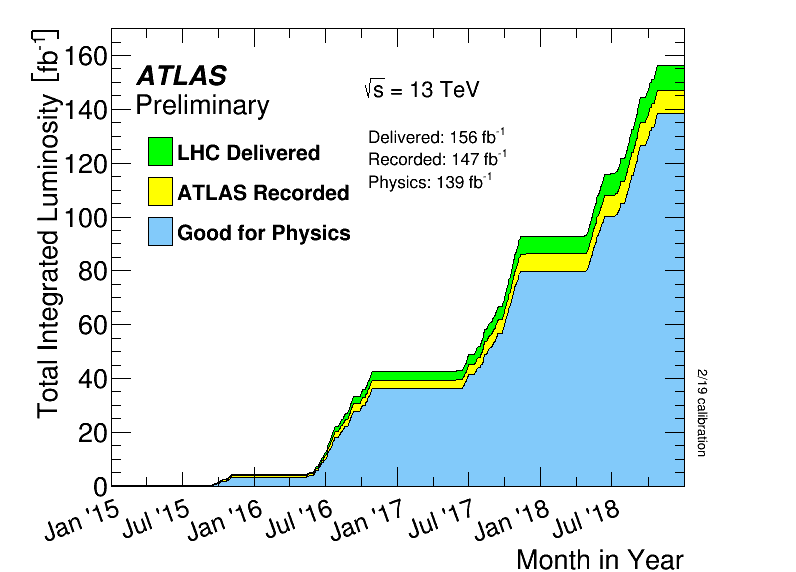
\includegraphics[width=.7\columnwidth]{../ThesisImages/LHCImages/ATLASLumi.png}
	\caption{Total integrated luminosity as a function of time delivered by the LHC(green), recorded (yellow) and declared good for physics analysis (blue) by the ATLAS detector throughout Run 2 consisting entirely of 13 TeV $pp$ collisions (figure from the ATLAS Collaboration).}
	\label{fig:ATLASLumi}
\end{figure}


\subsection{Pileup}

Increasing the luminosity is very beneficial for increasing the statistics needed when searching for rare events but it brings additional challenges as well.  Most interactions at any given detector are not hard-scatter events that correspond to poentially interesting physics cases but are instead soft collisions which create noise in the various detector experiments.  The LHC works hard to deliver as much data to the experiments as possible and delivers bunches of protons at a time.  It is possible for multiple pairs of protons to undergo these soft ineleastic collisions at a time.  The average number of interactions per bunch crossing, or pileup $\langle{\mu}\rangle$, for Run-2 was 33.7, shown in Figure \ref{fig:ATLASmeanIntperCrossing}. 
\begin{figure}[h!]
	\centering
	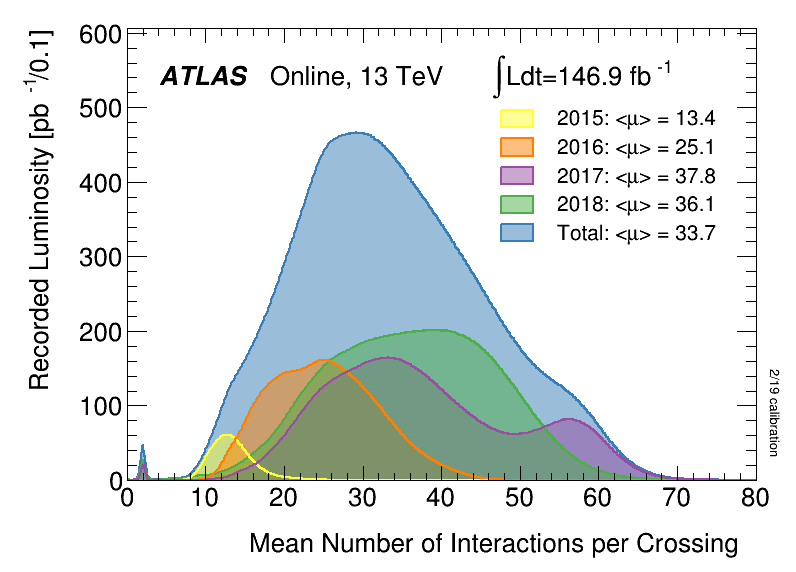
\includegraphics[width=.7\columnwidth]{../ThesisImages/LHCImages/meanIntperCrossing.png}
	\caption{Luminosity-weighted distribution of the mean number of interactions per bunch crossing for the entirety of Run 2 shown by individual years, 2015 (yellow), 2016(orange), 2017 (purple), 2018 (green), as well as an integrated total (blue) (figure from the ATLAS Collaboration).
	}
	\label{fig:ATLASmeanIntperCrossing}
\end{figure}
 The pileup must be accounted for when separating the tracks and energy deposited within a detector from an interesting hard-scatter event from the other soft collisions which occur at nearly the same time.  The difficulty of separating out one event from another can be seen in Figure \ref{fig:HighPileup} where there are 28 reconstructed verticies.  An extreme case of 65 reconstructed verticies is also shown in Figure \ref{fig:HighPileup2}.  As the LHC will continue to operate in the future at higher and higher luminosities the amount of pileup that will need to be dealt with will continue to increase.  
\begin{figure}[h!]
	\centering
	\includegraphics[width=.7\columnwidth]{../ThesisImages/LHCImages/28VertexPileup.png}
	\caption{ A candidate dimuon event ($Z\rightarrow \mu^+ \mu^-$) with 28 reconstructed verticies collected in 2018 with the ATLAS detector.
	}
	\label{fig:HighPileup}
\end{figure}

\begin{figure}[h!]
	\centering
	\includegraphics[width=.7\columnwidth]{../ThesisImages/LHCImages/65VertexPileup.png}
	\caption{ A candidate dimuon event ($Z\rightarrow \mu^+ \mu^-$) with 65 reconstructed verticies collected in 2017 with the ATLAS detector.
	}
	\label{fig:HighPileup2}
\end{figure}

\section{The ATLAS Detector}
Section:ATLAS
\begin{figure}[h!]
	\centering
	\includegraphics[width=\columnwidth]{../ThesisImages/LHCImages/AtlasDetector.png}
	\caption[Schematic of the ATLAS detector.]{Schematic of the ATLAS detector.\cite{ATLAS}
	}
	\label{fig:ATLASOverview}
\end{figure}

\begin{figure}[h!]
	\centering
	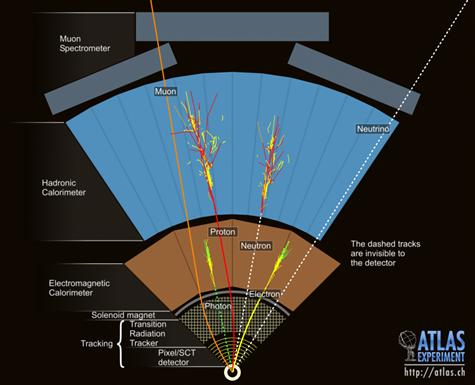
\includegraphics[width=\columnwidth]{../ThesisImages/LHCImages/ParticleInteractions.jpg}
	\caption[Cross section of a simulated ATLAS detector showing how various particles interact with ATLAS subsystems.]{Cross section of a simulated ATLAS detector showing how various particles interact with ATLAS subsystems.\cite{ParticleInteractions}
	}
	\label{fig:ATLASInteractions}
\end{figure}




\subsection{Coordinate System}
Coords
\begin{figure}[h!]
	\centering
	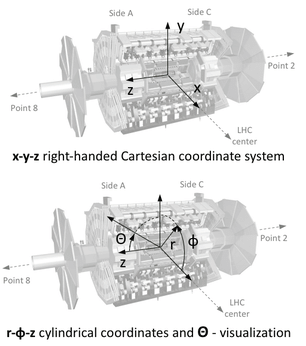
\includegraphics[width=0.5\columnwidth]{../ThesisImages/LHCImages/ATLASCoords.png}
	\caption[Coordinate system used in the ATLAS Collaboration.]{Coordinate system used in the ATLAS Collaboration.\cite{ATLASCoords}
	}
	\label{fig:ATLASCoords}
\end{figure}



\subsection{Magnet Setup}
\begin{figure}[h!]
	\centering
	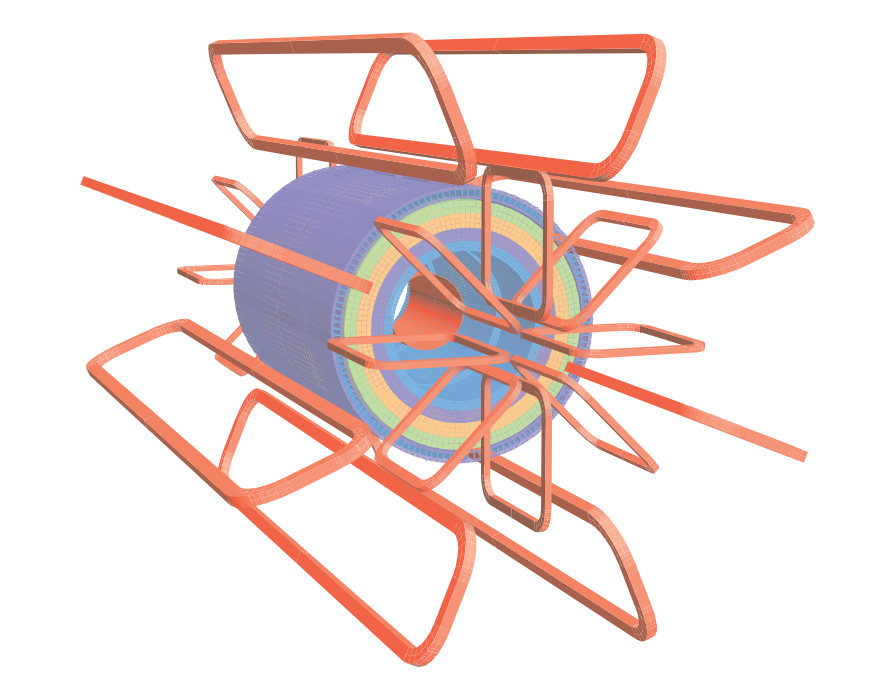
\includegraphics[width=0.5\columnwidth]{../ThesisImages/LHCImages/ATLASMagnetWinding.png}
	\caption[Schematic of the windings of the ATLAS magnet.]{Schematic of the windings of the ATLAS magnet.\cite{ATLAS}
	}
	\label{fig:ATLASMagnetWinding}
\end{figure}

%\subsection{SubDetectors}
\subsection{Inner Detector}

Inner
\begin{figure}[h!]
	\centering
	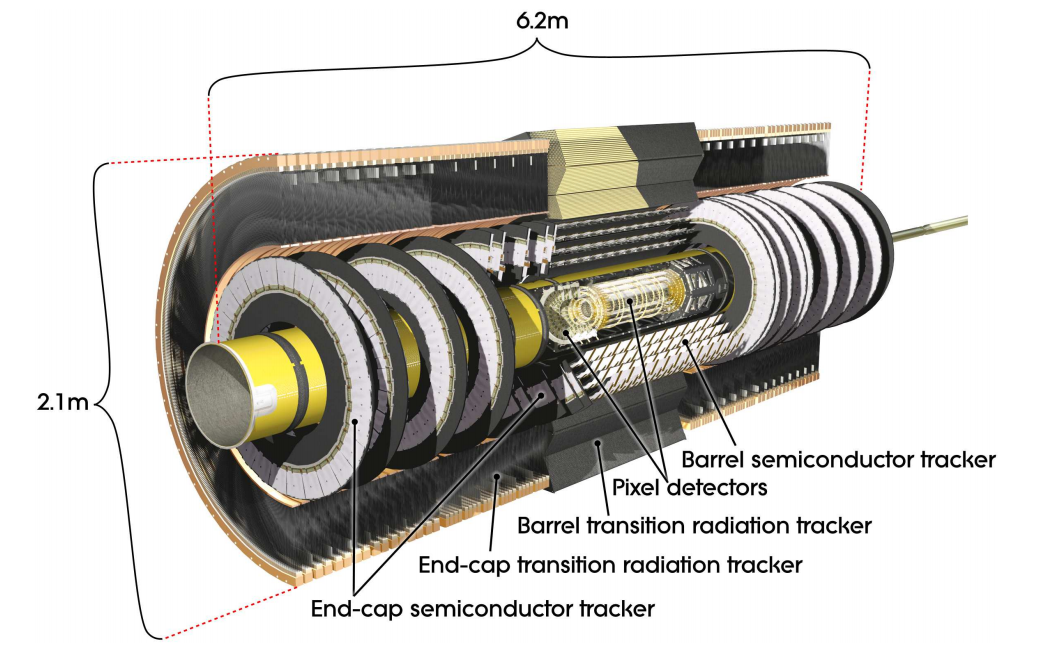
\includegraphics[width=0.5\columnwidth]{../ThesisImages/LHCImages/ATLASInnerDetector.png}
	\caption[Schematic of the ATLAS inner detector.]{Schematic of the ATLAS inner detector.\cite{ATLAS}
	}
	\label{fig:ATLASInnerDet}
\end{figure}


\begin{figure}[h!]
	\centering
	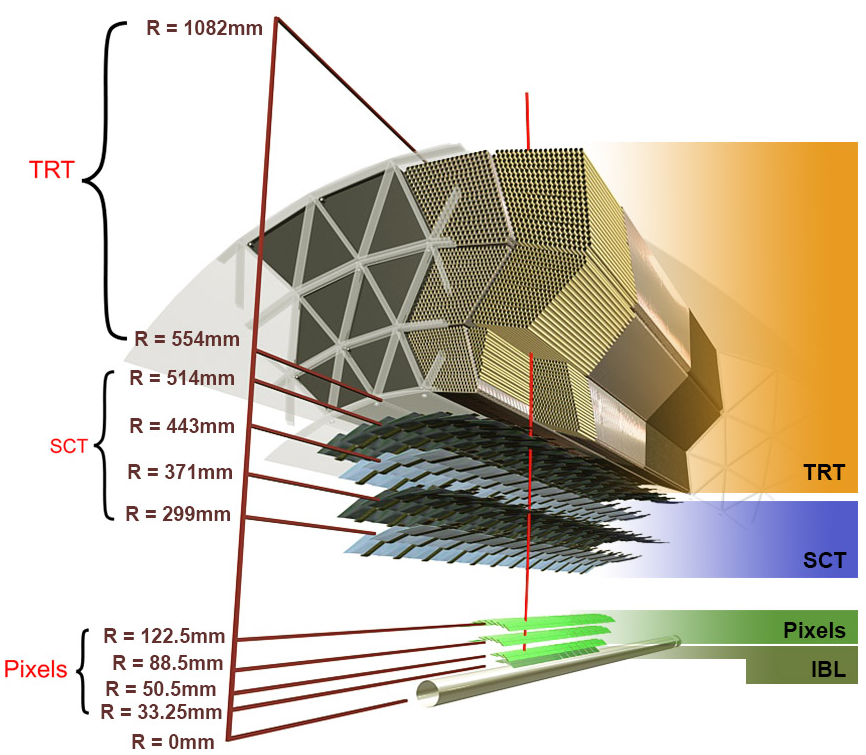
\includegraphics[width=0.5\columnwidth]{../ThesisImages/LHCImages/ATLASInnerStructure.png}
	\caption[Blown up schematic of the ATLAS inner detector with more detail.]{Blown up schematic of the ATLAS inner detector with more detail.\cite{ATLAS}
	}
	\label{fig:ATLASInnerDet}
\end{figure}

\subsection{Middle Layers, EMCal, HCal}
Middle chunks 
\begin{figure}[h!]
	\centering
	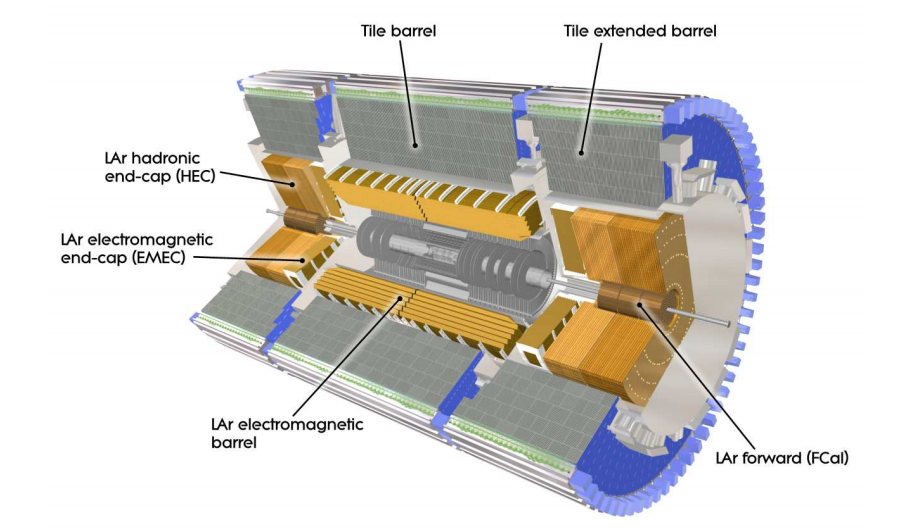
\includegraphics[width=\columnwidth]{../ThesisImages/LHCImages/ATLASCaloSystem.png}
	\caption[Schematic of the ATLAS hadronic and electromagnetic calorimeter systems.]{Schematic of the ATLAS hadronic and electromagnetic calorimeter systems.\cite{ATLAS}
	}
	\label{fig:ATLASCaloSys}
\end{figure}




\subsection{Muon Calorimeter}
Muons have to get picked up I guess
\begin{figure}[h!]
	\centering
	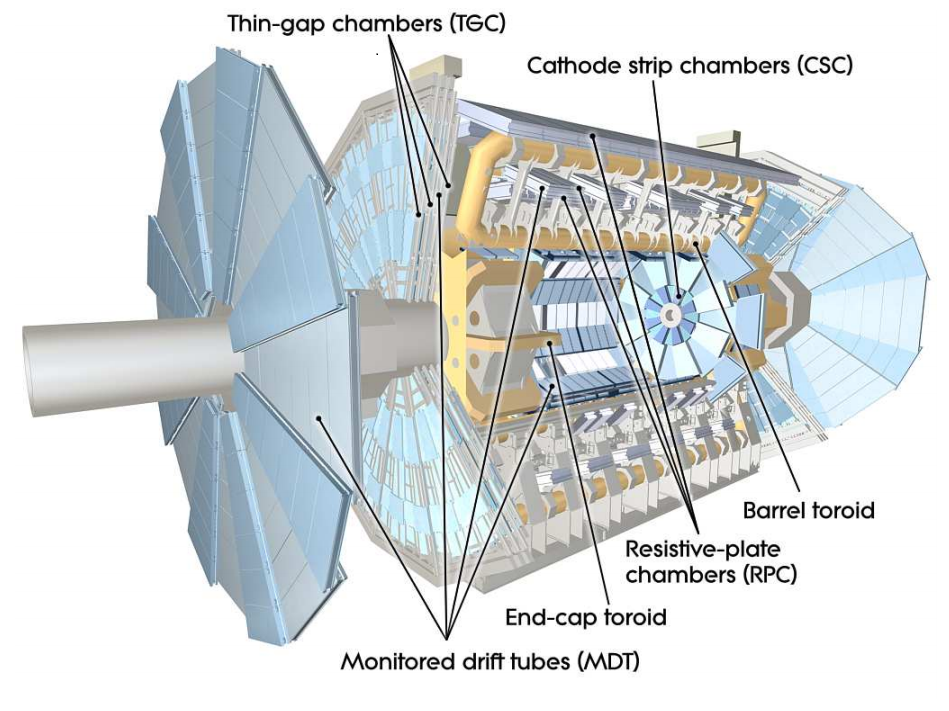
\includegraphics[width=\columnwidth]{../ThesisImages/LHCImages/ATLASMuonSystem.png}
	\caption[Schematic of the ATLAS muon detector.]{Schematic of the ATLAS muon detector.\cite{ATLAS}
	}
	\label{fig:ATLASMuonSys}
\end{figure}

\subsection{Trigger and Data Acquisition}
All of these subsystems lead into actual data farm
\begin{figure}[h!]
	\centering
	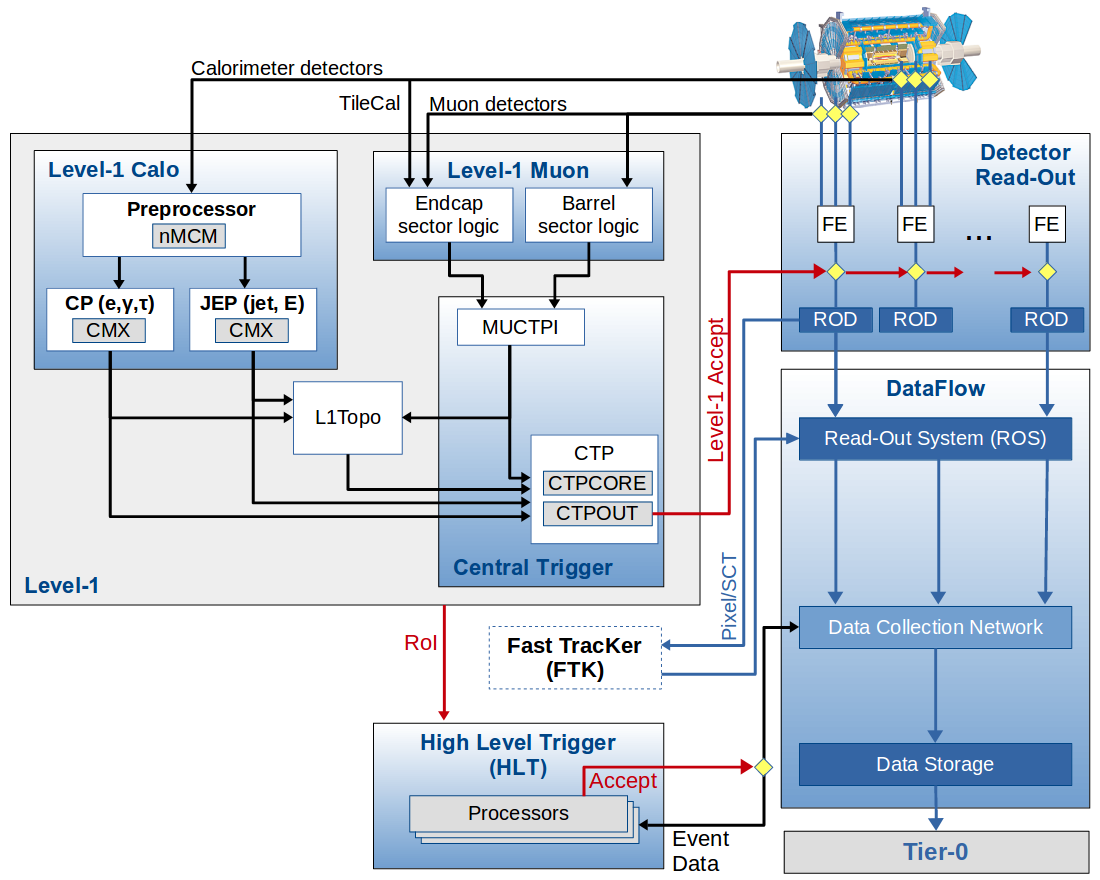
\includegraphics[width=\columnwidth]{../ThesisImages/LHCImages/ATLASTDAQR2.png}
	\caption[Flow diagram of the ATLAS trigger and data acquisition system used in Run 2.]{Flow diagram of the ATLAS trigger and data acquisition system used in Run 2.\cite{ATLASTDAQ}
	}
	\label{fig:ATLAStdaq}
\end{figure}

\subsubsection{L1Calo}
\subsubsection{HLT}
%\subsubsection{Data Farm Information}
%\subsubsubsection{Trigger Rates}
%\subsubsubsection{Amount of Data}


%%%%%%%%%%%%%%%%%%%%%%%%%%%%%%%%%%%%%%%%%%%%%%%
%%%%%%%%%%%%                                                                                                   %%%%%%%% 
%%%%%%%%%%%%                           BEN                                                                  %%%%%%%% 
%%%%%%%%%%%%                                                                                                   %%%%%%%% 
%%%%%%%%%%%%%%%%%%%%%%%%%%%%%%%%%%%%%%%%%%%%%%%
%The particle physics program at CERN uses some of the most complex machines ever built, and have required the efforts of thousands of people to design, commission, and maintain.  This section outlines the systems which are used to provide the collisions and measure their products.
%
%\section{The Large Hadron Collider}
%
%The Large Hadron Collider (LHC) is the worlds largest and most powerful particle accelerator, at over 27\,km in circumference and capable of accelerating protons a center of mass energy of 13\,TeV.  It is located 100 meters underground along the French-Swiss border at CERN, just outside Geneva, Switzerland.  The beams are brought to collisions at different points along the ring to four major experiments: ATLAS~\cite{ATLAS}, CMS~\cite{CMS}, ALICE~\cite{ALICE}, and LHCb.\cite{LHCb}
%
%Protons in the LHC start as hydrogen gas which is ionized, the protons of which are accelerated to 50\,MeV by the LINAC2 linear accelerator.  From here, particles are accelerated in a series of circular accelerators of increasing size, starting with the Proton Synchrotron Booster which raises their energy to 1.4\,GeV.  This is followed by the Proton Synchrotron (PS) (25\,GeV) and Super Proton Synchrotron(SPS) (450\,GeV), after which proton bunches are finally injected into the LHC where they are ramped up to their final collision energy.  For Run 1, the LHC operated $\sqrt{s}$ = 7 and 8\,TeV, while in the ongoing Run 2 at $\sqrt{s}$ = 13\,TeV.  The CERN accelerator complex is shown in Figure~\ref{fig:AcceleratorMap}.
%
%\begin{figure}[h!]
%	\centering
%	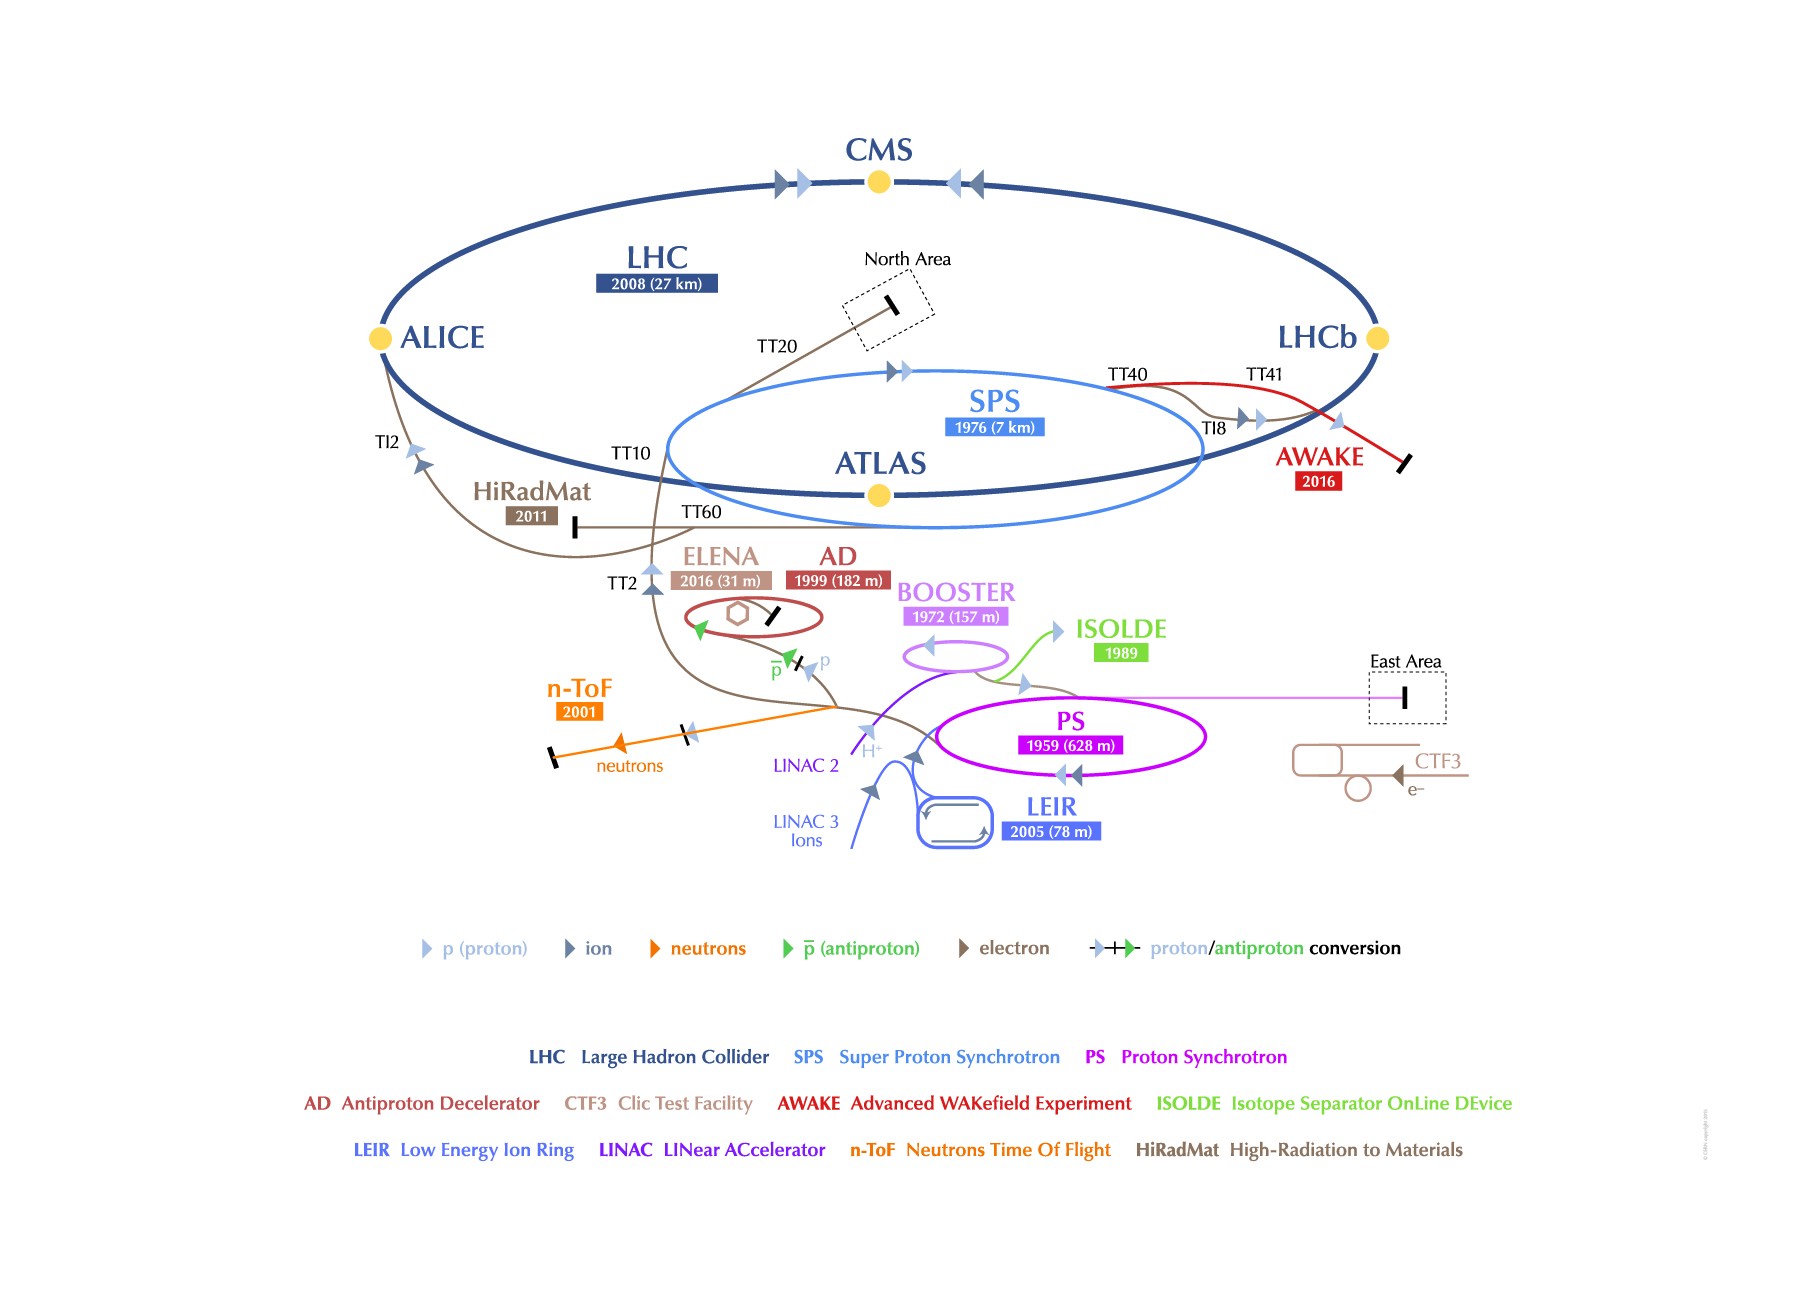
\includegraphics[width=\columnwidth]{figures/Detector/CERNAcceleratorComplex.jpg}
%	\caption{Schematic of the CERN accelerator complex.\cite{DeMelis:2119882}
%	}
%	\label{fig:AcceleratorMap}
%\end{figure}
%
%\subsection{Bunches and bunch trains}
%
%The LHC operates at a radio frequency (RF) of 400\,MHz which can be filled with bunches every 10 RF buckets for a separation of 25\,ns between bunches.\cite{Boussard:410377}  During Run 1 and the early part of Run 2 the LHC operated with 50\,ns spacing to reduce the effect of the electron cloud, but moved to the design spacing of 25 ns for the remainder of Run 2 data taking at the insistence of the detector collaborations.  This spacing, coupled with the $\sim27$\,km circumference of the LHC, means there are 3564 bunches which could be filled in the ring at any time.  In practice the LHC never fills all of these bunches at once, but instead the bunches are organized into $trains$.
%
%Bunch trains are groups of sequentially filled bunches in the machine and are driven by the design of the PS and SPS rings.  For a typical 2016 run, a single injection from the PS to the SPS was 72 sequential bunches, while the SPS transferred 288 bunches (4$\times$72) at a time over to the LHC.\cite{Bartmann:IPAC2017-TUPVA007}  The gaps between each of these bunches are driven by the kicker magnet rise times for each of these systems.  The minimum kicker times for the PS and SPS are 200\,ns and 800\,ns respectively, so each 72 bunch train is separated by 8 empty bunches, and each grouping of 288 is separated by 32 empty bunches.  The filling scheme also includes an abort gap, a space of approximately 100 empty bunches which is used in the case that the beam needs to be redirected to the beam dump.  In total, the number of filled bunches in the machine caps out around 2800 at a time.
%
%While the overall luminosity can be directly increased by upping the number of bunches in the machine at one time, the LHC has also tested other filling schemes which reduce the number of filled bunches but increase the charge in each bunch, or decrease the beam emittance, leading to a higher instantaneous luminosity and overall integrated luminosity.
%
%\section{The ATLAS Detector}
%
%The ATLAS detector is a multipurpose physics detector, located at Point 1 on the LHC ring near the main CERN site.  ATLAS weighs in at around 7000 tons, and is 44\,m long and 25\,m in diameter.  The detector is composed of multiple layers which measure their own unique portions of the collision products, which are described in the following section.  Figure~\ref{fig:AtlasDetector} shows how these systems are laid out.
%
%\begin{figure}[h!]
%	\centering
%	\includegraphics[width=\columnwidth]{figures/Detector/AtlasDetector.png}
%	\caption{A cutaway view of the ATLAS detector showing the various components.\cite{ATLAS}
%	}
%	\label{fig:AtlasDetector}
%\end{figure}
%\subsection{Coordinate System}
%
%The ATLAS experiment uses a right-handed coordinate system, with the origin at the nominal interaction point (IP) in the center of the detector.  The x-axis points from the IP towards the center of the LHC ring, and the y-axis points upward towards the surface.  ATLAS uses a cylindrical coordinate system which defines a radial distance $r = \sqrt{x^2+y^2}$ and azimuthal angle $\phi$ around the z-axis.  Instead of using the polar angle from the beamline $\theta$, pseudorapidity is typically used, defined as $\eta = -\ln{(\tan{\frac{\theta}{2}})}$.
%
%Massive objects, such as jets, are measured to have a rapidity defined as $ y = \frac{1}{2}\ln{\frac{E+p_z}{E-p_z}}$.  In the limit where $\pt \gg m$, as is often the case in this search, $y \approx \eta$, meaning that the rapidity of a jet and its detector location given by pseudorapidity are approximately interchangeable.  Differences in rapidities are Lorentz-invariant under z-axis boosts, making them useful for measuring if two jets are back-to-back in their rest frame.
%
%\subsection{Magnet System}
%
%ATLAS is composed of four separate magnets: one central solenoid encompassing the ID, one barrel toroid, and two endcap toroids.  The central solenoid provides a 2.0\,T magnetic field and is responsible for bending charged particle tracks near the IP to measure their momentum.  The namesake toroids provide a peak field of 4.0\,T, bending muons in a different plane than the solenoid field does to improve their momentum measurement.
%
%\subsection{Inner Detector}
%
%The ATLAS Inner Detector (ID) is comprised of three different subsystems: the silicon pixel layers (including the Insertable B-Layer (IBL) new in Run 2), the semiconductor tracker (SCT), and transition radiation tracker (TRT).  In total, the system covers the angular range $|\eta|<2.5$.  Information from all three subsystems is used to reconstruct tracks down to \pt = 0.4\,GeV.\cite{IDPerf}
%
%\subsubsection{Pixel and Semiconductor Trackers}
%
%The pixel detector system is composed of four concentric layers of silicon pixels, providing multiple high-resolution hits for charged particles traveling through.  The closest layer to the beampipe, the IBL, was added during Long Shutdown 1 (LS1) before the start of Run-2 operations.  At only 3.3\,cm away from the beamline, this additional tracking layer greatly improved the efficacy of tracking algorithms by an additional hit for tracks passing through multiple layers, and allowing for better resolution of secondary decay vertices, such as those originating from b-quarks.  The IBL also contains newer technologies than the rest of the pixel system which allow it to withstand the harsh radiation close to the beampipe.  This will allow the IBL to continue performing well as the innermost layer of the old pixel system degrades due to radiation, allowing for the maintenance of the current tracking performance.
%The SCT uses silicon microstrips and sits just outside the pixel system.  It is comprised of four barrel layers and 18 endcap disks (9 on each side of the detector), and range from 30 to 51\,cm from the beamline, adding additional position information for track finding.
%
%\subsubsection{Transition Radiation Tracker}
%
%The TRT operates on a very different principle than the other two tracking systems, taking advantage of the energy emitted when high energy particles transition between media with differing indices of refraction.  It is comprised of nearly 300,000 polyimide straws with an external aluminum layer and central gold-plated, tungsten wire at the center of each 4mm diameter tube.  The straws are filled with a gas mixture of Ar, CO$_2$, and O$_2$, and are ionized either by charged particles passing through or by emitted transition radiation.  Each straw hit provides additional 2-D hit information for track finding, as well as acting as a discriminant in electron identification.
%
%The TRT is scheduled to be removed as part of the ATLAS Phase-II upgrade starting in 2025, as the pileup conditions in Run 4 are expected to create TRT occupancies near 100\%, significantly degrading the performance of the system. The average TRT occupancy as a function of the number of interactions per crossing is shown in Figure~\ref{fig:TRTOccupancy}.  
%
%\begin{figure}[h!]
%	\centering
%	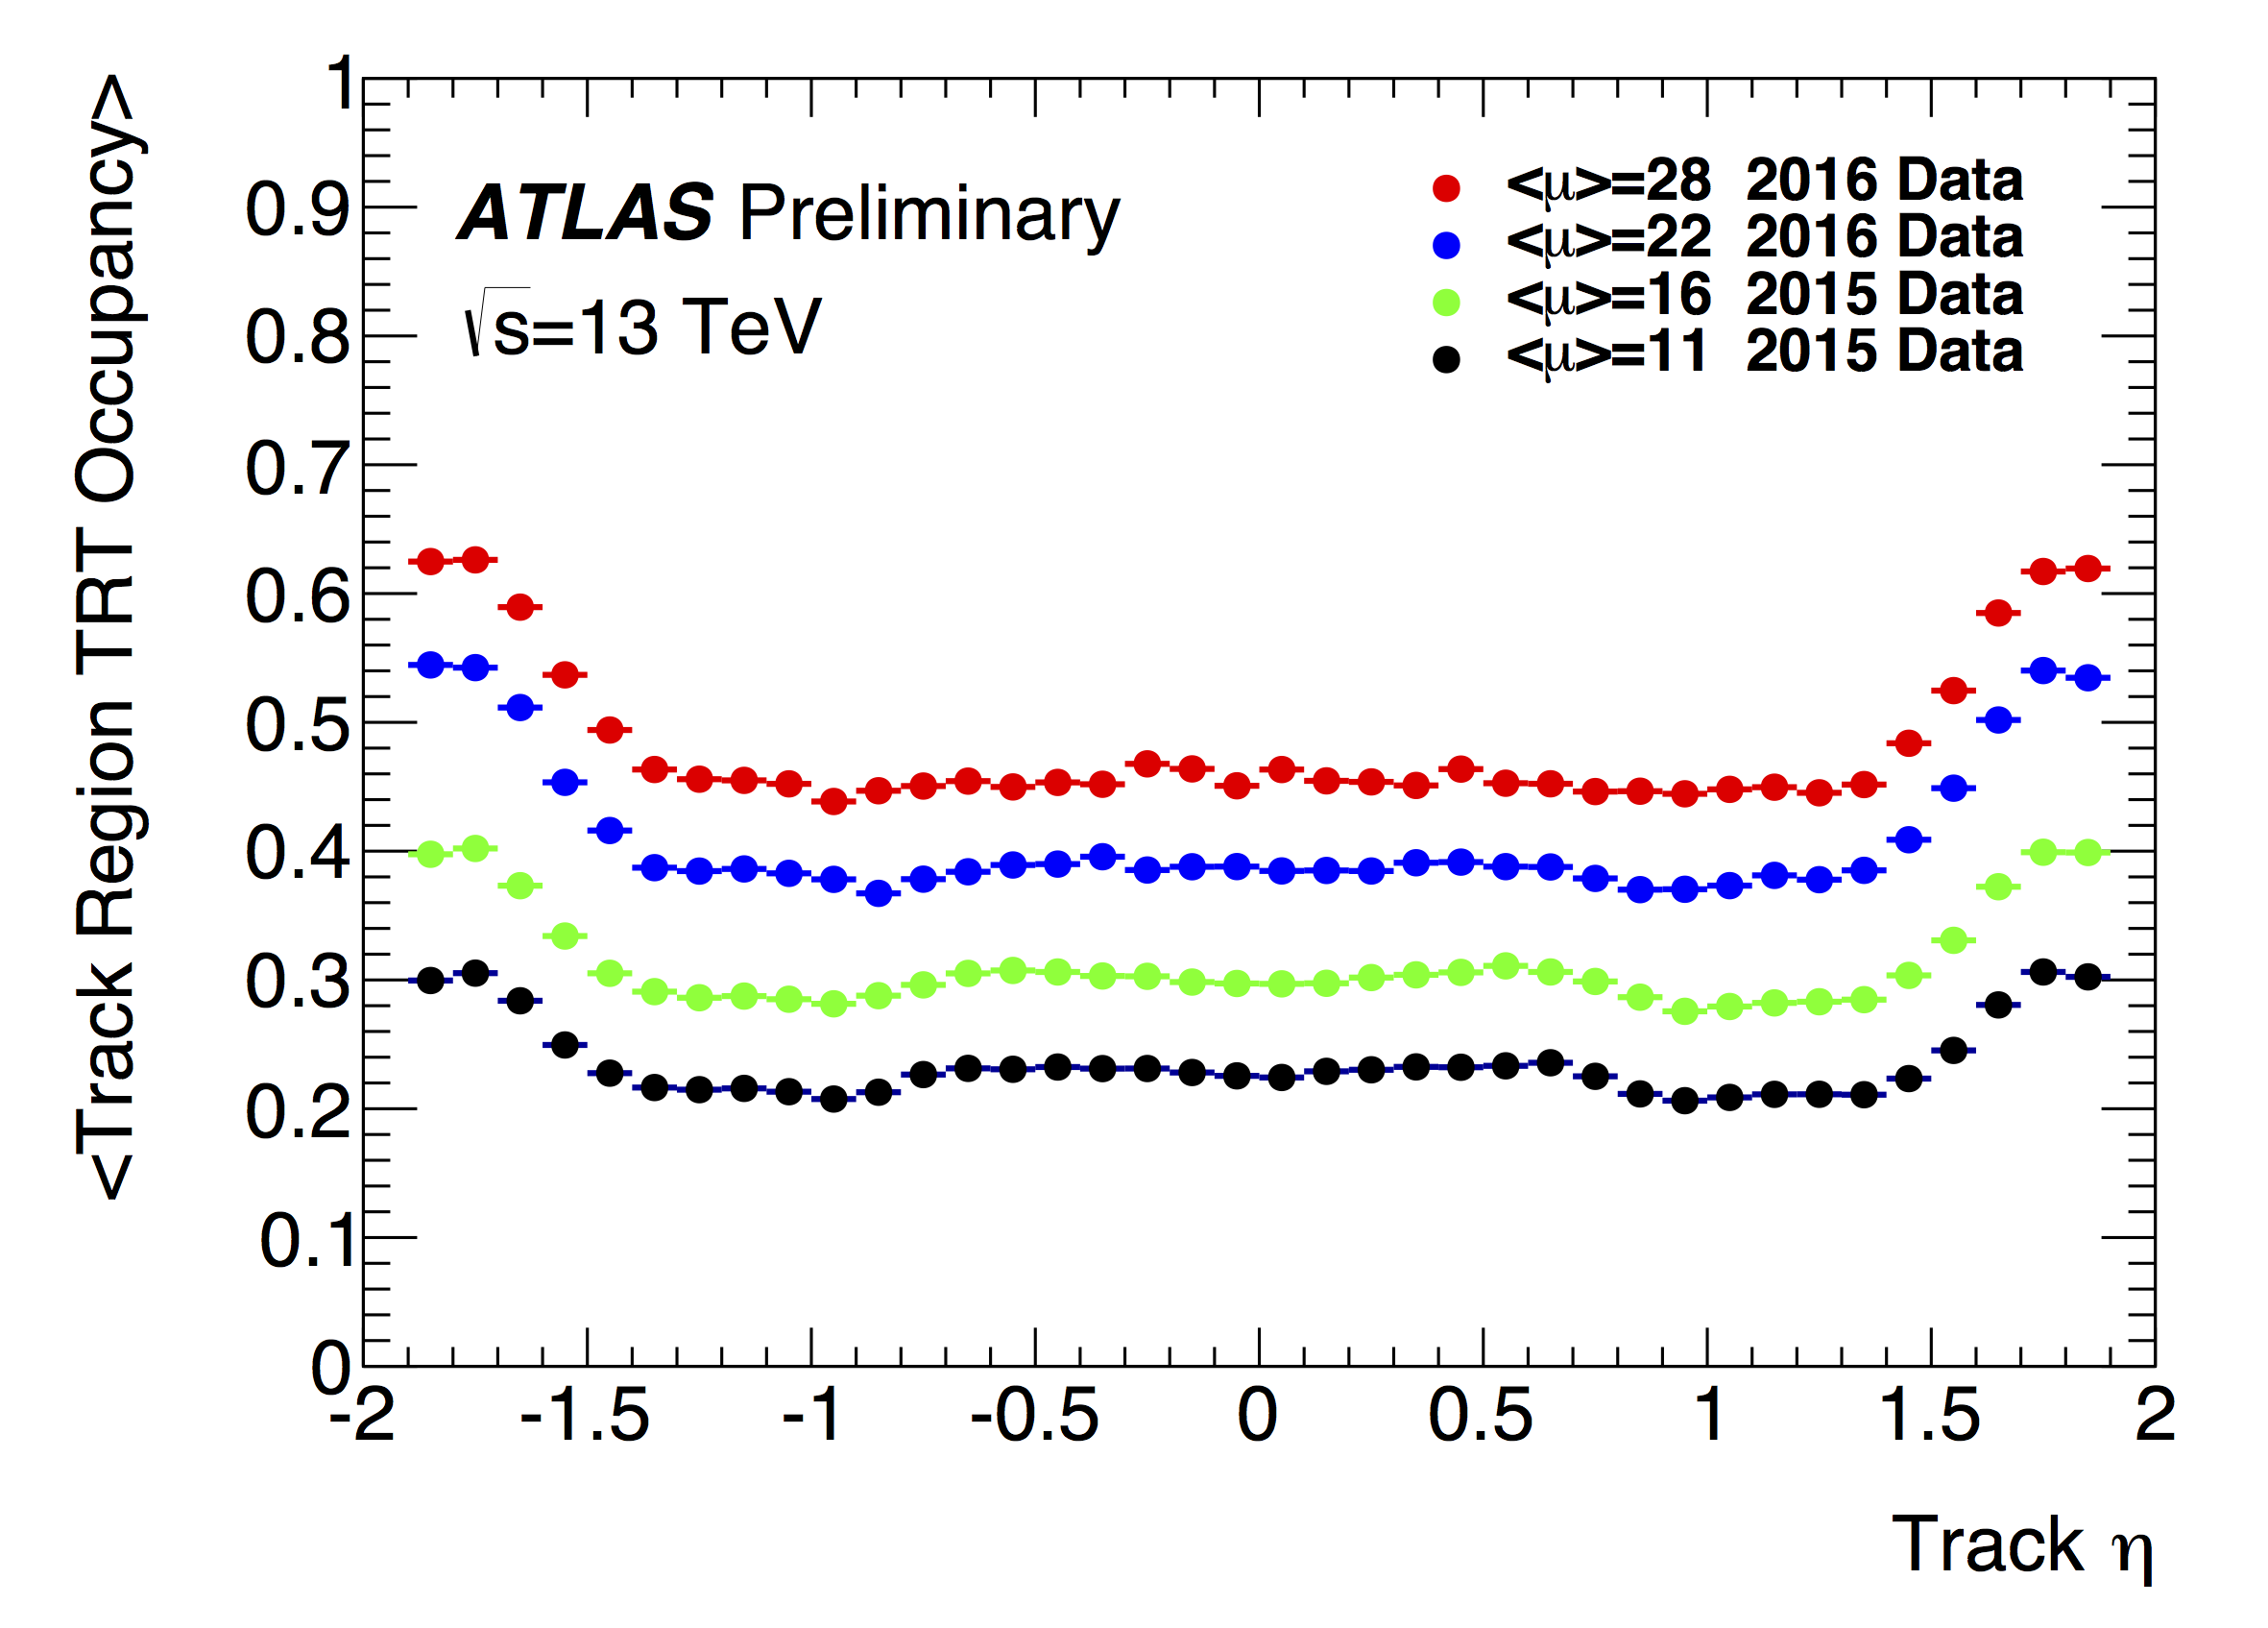
\includegraphics[width=0.6\columnwidth]{figures/Detector/TRTOccupancy.png}
%	\caption{Average track region TRT occupancy as a function of track $\eta$ using data taken during the 2015 and 2016 ATLAS runs for four different values of the average interactions per bunch crossing.
%	}
%	\label{fig:TRTOccupancy}
%\end{figure}
%
%\subsection{Calorimeters}
%
%ATLAS uses two different types of calorimeters to measure the energies of leptons, hadrons, and photons.  First is the liquid argon (LAr) electromagnetic calorimeter, which captures most of the energy from EM showers.  Second is the steel-scintillator Tile calorimeter which captures the energy from hadronic showers.  Optimal performance of the calorimeter systems under challenging conditions is vital to nearly every physics signature ATLAS searches for.  The system has nearly hermetic coverage in $\phi$ but is made up of several overlapping systems and varying thicknesses of material in $\eta$, and so special care must be taken to accurately calibrate the detector response in each region of the detector.
%
%The journey from calorimeter hits to the eventual trigger is discussed in detail in Chapter~\ref{ch:Calorimetry}.
%
%\subsubsection{Electromagnetic Calorimeter}
%
%The EM calorimeter uses liquid argon as an active medium, a choice motivated by the need for radiation-hardness, especially over the 30+ year run time of the LHC.  The calorimeter is composed of accordion shaped absorbers of lead with steel backing, with liquid argon flowing between and copper electrodes which measure the energy deposited.
%
%The LAr calorimeter is a sampling calorimeter, meaning that only a small fraction of the total energy from a particle traversing it is actually measured.  The power of an absorbing material is given by its radiation length ($X_0$), the distance an electron must travel in that material for its energy to be reduced by a factor of $\frac{1}{e}$.  Liquid argon is not dense enough as a medium to fit in a reasonable size calorimeter, and so lead (with a radiation length 20$\times$ shorter) is used to slow down the particles.  The EM calorimeter contains enough material to fully contain all but the largest electromagnetic showers, typically 25-30 interaction lengths depending on the region of the detector.  The actual pulse observed in the calorimeter is created when charged particles, showering from interactions in the absorber layers, cause the LAr to ionize and then release electrons which are accelerated by an electric field to the electrodes to become the calorimeter pulse.  The amount of energy actually measured by the LAr is much less than the total shower energy, and so it must be scaled back up by comparing the behavior of particles using test beam data where the incoming particle energy is well known.
%
%The EM Barrel covers the central region out to $|\eta|<1.475$, and two endcaps cover the range $1.375<|\eta|<3.2$.  The calorimeter is divided up into four layers of varying granularity, the first of which is the presampler.  This layer is closest to the inner tracker and has no absorber material in it, but instead is used to measure the amount of energy which has dissipated due to interactions with the material in the inner detector before it reaches the calorimeters.  The other three layers vary in thickness and granularity, and the values from each of these layers help determine the shape evolution of the shower as it progresses through the calorimeter, an important tool for electron/photon identification.  These pulses are read out and given to the level-1 trigger at coarse level, and if an event passes the trigger they are passed with full granularity to the high-level trigger.
%
%\subsubsection{Hadronic Calorimeter}
%
%Situated immediately outside the EM calorimeter, the hadronic calorimeter systems capture the remaining energy from hadrons which have already deposited a fraction of their energy in the EM layers.  The depth of material is characterized by the number of nuclear interaction lengths, the distance a hadron travels before undergoing an inelastic collision.  The depth varies as a function of $\eta$, but the hadronic calorimeters typically comprise 8-12 interaction lengths, enough to stop all but the most powerful showers.  In the barrel region, it is comprised of steel absorbing layers and scintillating polystyrene tiles, and the deposited energy is measured by molecular excitations in the scintillator emitting UV light which is then read out by photomultiplier tubes (PMTs).  The barrel systems covers the region $|\eta|<1.7$, but a different, more radiation-hard technique is required for the more forward regions.
%
%The Hadronic Endcap (HEC) covers the range $1.5<|\eta|<3.2$, and operates in largely the same manner as the EM systems.  Instead of the lead-steel combination of the EM layer, the HEC uses much thicker copper layers as the absorbers, with LAr still acting as the active medium.  The forward calorimeter (FCAL) covers the range $3.1<|\eta|<4.9$ and uses a combination of copper and tungsten plates as the absorbers.  Overall the hadronic calorimeters are much coarser than their EM counterparts, with a granularity of 0.1$\times$0.1 ($\Delta\eta\times\Delta\phi$) in the region $|\eta|<2.5$, and $0.2\times0.2$ in the forward regions.  
%
%\subsection{Muon Spectrometers}
%
%Muons interact very little with the calorimeters in ATLAS, leaving behind only tracks in the inner detector before they reach the outermost systems in ATLAS, the muon spectrometers.  In the muon systems, ATLAS's namesake toroids bend the tracks of passing muons to determine their momenta.  The muon system uses different technologies in the barrel and endcap regions, as well as different systems for triggering and momentum measurement.
%
%In the central region, monitored drift tubes (MDTs) are used to measure the tracks, and thus the momenta, of muons, while resistive plate chambers (RPCs) are used for triggering.  This split is required because of the long drift time of the MDTs of ~700\,ns, which is outside of the window the level-1 trigger system can use.  To deal with the higher backgrounds in the forward regions, cathode strip chambers (CSCs) are used for momenta measurements and thin-gap chambers (TGCs) are used for triggering.
%
%The muon system operates under the assumption that all other particles will be fully absorbed in the calorimeter layers, and thus any detected particles in the region must be muons.  However, in the case of very high-\pt jets some of the energy can "punch through" the calorimeters and register hits in the muon system.  This effect must be compensated for and is discussed later in the context of jet calibration.
%
%\subsection{Forward Detectors}
%
%Further down the beampipe from the IP are the various forward detectors for ATLAS which are primarily used for luminosity and cross-section measurements.  LUCID (LUminosity measurement using Cerenkov Integrating Detector) sits 17\,m down from the IP and consists of quartz fiber bundles connected to PMTs which detect Cherenkov radiation as charged particles pass through the quartz.  The multiplicity is proportional to the amount of interactions taking place at the IP, and is therefore used to measure the instantaneous luminosity.  ALFA (Absolute Luminosity For ATLAS) uses Roman Pots 240\,m from the IP to detect protons at angles very close to the beamline; ALFA is used in dedicated runs to measure the total proton-proton cross-section.  ZDC (Zero Degree Calorimeter) sits 140\,m from the IP and is used to measure the amount of neutral particles (neutrons and photons) left as beam remnants once the rest of the beam has been bent away by the steering magnets of the LHC; this information is used as a minimum-bias trigger for ATLAS, and as a centrality measurement for heavy-ion collision data.  Finally, AFP (ATLAS Forward Protons) is new for Run 2, primarily focusing on diffractive physics in special low-luminosity runs.
%
%\subsection{Trigger and Data Acquisition}
%During nominal operations, the LHC provides collisions at a rate of 40\,MHz, or an event every 25\,ns.  As each event is slightly under 2\,MB of data, this represents an extraordinary amount of information, and is far more than could be conceivably be written to disk, much less properly analyzed.  In order to reduce the data rate to a manageable level, and to ensure that only the events with the most interesting physics are saved, a two-tiered trigger system is used.
%\subsubsection{Level-1 Trigger}
%The level-1 (L1) trigger is hardware based, making decisions on whether or not to keep an event within 2.5\,$\mu$s.  For Run-2 operation, the L1 trigger reduces the event rate to a maximum of 100\,kHz.  The L1 trigger is made up of several subsystems which bring together decisions from different areas of the detector to make a final decision on whether or not to keep an event.
%
%The L1 calorimeter trigger (L1Calo) uses information from the EM and hadronic calorimeters in the form of rough 0.1$\times$0.1 ($\eta\times\phi$) trigger towers.  From this information, candidates for jets, electrons/photons, and taus are constructed and passed along as regions of interest (RoI) to the next stages in the trigger telling the type of object, its transverse momentum as measured at L1, and its location in the detector.  The amount of global missing transverse energy (MET) is also calculated and used as part of the trigger signature.  The L1Muon system uses a coincidence of hits in the RPCs and TGCs to identify muon candidates.  Since precision momentum information from the MDTs and CSCs takes too long for the L1 decision, the muon momentum is roughly estimated using the hit pattern, and then marked as being above one of a set number of \pt thresholds.
%
%Within each system, a list of pre-determined triggers are compared against the RoIs found in the event.  For example, the muon system has triggers for muons above 20\,GeV (L1\_MU20) as well as for two muons above 6\,GeV (L1\_2MU6).  The list of all triggers passed in each system is passed along to the Central Trigger Processor (CTP) where the final determination on whether or not to save an event is made.
%
%RoIs from both L1Calo and L1Muon are then sent to the L1 Topological trigger. (L1Topo)  Newly commissioned in 2016, L1Topo allows for more advanced combinations of trigger objects from the two systems, including operations such as invariant mass, angular separation between objects, and transverse mass.\cite{L1Topo}  This additional processing step greatly reduces the background rates for certain processes, allowing for much lower energy thresholds when using objects triggered from L1Topo.  Similar to L1Calo and L1Muon, the list of triggers passed by an event is passed along to the CTP.
%
%The CTP is the final stage of the L1 trigger.  It receives a list of all passed triggers from the other subsystems and compares it against an L1 trigger menu.  The trigger menu determines which triggers should be turned on or off during a given run, as well as the prescale, or rate reduction, rates for triggers.  Triggers with lower energy thresholds are often prescaled, meaning that only a fraction of events that pass a given trigger are kept.  For example, a physics menu item with a prescale of 20 will have only 1 out of 20 events that pass the trigger saved, while the other 19 times the event is not saved unless some other trigger is also passed and and marks the event for saving.  The L1 trigger menu evolves over the course of time as well as within a single physics run, changing the prescales of physics items to keep the rate of saved data as close to 100\,kHz as possible as the instantaneous luminosity decays.  If the CTP determines that an event passes at least one trigger after prescaling, then the event is saved.  At this point a level-1 accept signal is sent which triggers the readout of the full granularity detector data.  The result of which triggers were passed at the CTP, along with the RoIs, are then passed along to the high-level trigger.
%
%\subsubsection{High Level Trigger}
%
%Events passing the L1 trigger are fed to the High-Level Trigger (HLT), which uses the full detector readout and granularity to measure physics quantities at close to offline precision.  For Run 2, the HLT accepts events at nearly 100\,kHz and reduces this rate down to 1\,kHz for the general physics stream.  The HLT runs on a general computing cluster with thousands of cores and uses much more complex software algorithms for event analysis, such as b-tagging and anti-$k_t$ jet clustering.
%
%HLT trigger chains are seeded by an matching relevant L1 trigger.  For example, the single-jet trigger HLT\_j380 is seeded by the L1 trigger L1\_J100.  As events can pass multiple trigger thresholds and types, multiple HLT algorithms can be run on a single event.  Each HLT item corresponds to a chain of processing steps which are optimized to reject events as early as possible, using the full readout and precision processing steps only on the most likely candidates.  There are several different types of HLT chains which are used, including primary chains, the unprescaled standards used by most analyses, supporting chains, which are typically prescaled and are used mainly for determining backgrounds for other analyses in regions which can not support an unprescaled trigger, and monitoring chains, which readout only a small portion of the whole detector and are used to check the performance of specific subsystems.
%
%The debug stream includes events which are unable to be processed in the HLT, either due to them timing out after taking too long to process, or because of some issue which caused a crash.  All events which cause errors in the HLT are saved to the debug stream to ensure no interesting events are lost, and to troubleshoot which algorithms are problematic.  The debug stream typically only contains a handful of events per run, but on occasion HLT farm crashes have caused hundreds of thousands of events to be saved to it.  ATLAS also uses a data scouting stream which supports lower threshold physics searches by giving them drastically increased event rate in exchange for saving only a small portion of the event data.  This stream is used by the ATLAS Trigger Level Analysis (TLA) to look at dijet events in the invariant mass range below the reach of the standard dijet search.
%
%\subsection{Dead Time}
%
%The ATLAS detector is limited in how many events in can process in a given amount of time, leading to "dead time" for the detector when collisions are occurring and the detector is operating nominally, but events are unable to be saved.  The first type is referred to as simple dead time, which occurs after every L1Accept and takes about 100\,ns, or 4 bunch crossings.  During this time the detector is transferring the full readout to the front end buffers for processing in the HLT and can not save any other events.  The second type is complex dead time which comes about from the limited size of these readout buffers for individual subsystems and the rate at which data can be sent off-detector.  Complex dead time limits the number of accepted events in a given period of time; if too many events occur too quickly, the readout buffers fill up and events must be vetoed until there is space for another event in the buffer.  The complex dead times are controlled by four "buckets" which are adjustable between runs depending on the requirements of the different hardware subsystems, characterized by a max number of L1Accepts in a given number of BCs.  For example, 15/430 means that up to 15 events can be saved within a window of 430 BCs, and triggers are put on hold until the rate drops down below this level.
%For the dataset used in this analysis, ATLAS recorded data with 92\% efficiency. The total amount of dead time varies based on the luminosity, but typically covers $\sim3\%$ of collision time.  The remaining inefficiency comes from reducible sources such as detector errors which send a busy signal and hold triggering while the system fixes an issue or resets a component.
%
%\subsection{Data Processing}
%
%Events which are accepted by the HLT are written to disk and are passed to the ATLAS Tier-0 computing facility at CERN, where the detector readout is transformed from raw data into the physics objects that will eventually be used for analyses.  Immediately after a run is taken, the express stream (a small subset of the full physics data stream) is run through what is known as the calibration loop, a $\sim48$ hour process in which the geometry and conditions for the run are calculated to properly process the whole dataset.
%
%Once calibration is complete, the data enters bulk reconstruction where the full dataset is run through the standard ATLAS software to change the data from raw detector readout to containers which describe objects such as electrons and jets, or more granular objects such as track-candidates or calorimeter clusters.  This data format is known as xAOD, or Analysis Object Data.  This dataset is then duplicated around the world to the various computing facilities around the globe.  From here, the data is run through the Derivation Framework.
%
%To prevent analyses from needing to run over the entire ATLAS dataset, each group of analyses sharing a similar signature creates a specialized derivation which skims through the full dataset and only keeps events which are likely to be relevant to the analysis, and allows groups to remove unneeded data containers, or to create their own data containers which are not part of the standard set.  For example, the derivation which the dijet analysis uses keeps only events which pass one of the single- or multi-jet HLT chains, and gets rid of muon and electron data as those objects are not used in any way in the analysis.  The typical derivation is only$\sim1-2\%$ of the full AOD in size, making it much more manageable for analyses to run their search over.  These derived AODs (DxAODs) are then duplicated to multiple places in the CERN computing grid and become available for analysis use.  The main physics stream for ATLAS recorded 1.7 billion events in 2015 and 5.4 billion in 2016, comprising some 6.2 petabytes of raw data, making running over the full dataset exceedingly difficult!